% expect: native match>=0.95
\usetikzlibrary{matrix,positioning}
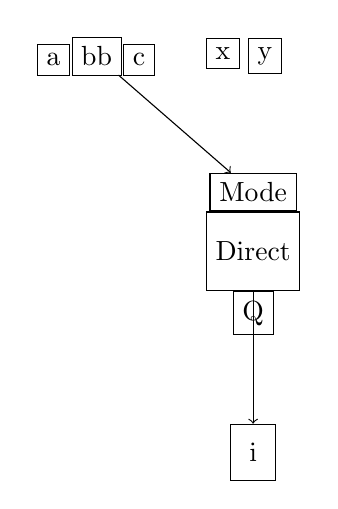
\begin{tikzpicture}
\matrix[matrix of nodes, nodes={draw, line width=0.2pt}, column sep=0.025cm](O1) { a & bb & c \\ };
\matrix[right=0.4cm of O1, matrix of nodes, nodes={draw}, column sep=1mm](O2) { x & y \\ };
\matrix[below left = 1cm and -1.45cm of O2, matrix of nodes, nodes={draw}](H) { |[name=mode]| Mode \\ |[minimum height=1cm,name=dir]| Direct \\ |(q)| Q \\ };
\matrix[below = 1cm of H, draw](I) { \node {i}; \\ };
\draw[->] (O1-1-2) -- (mode);
\draw[->] (dir) -- (I);
\end{tikzpicture}
